% Source: fig2-drawio/fig2-task-grounded-intervention.drawio.
\begin{figure}[htbp]
  \centering
  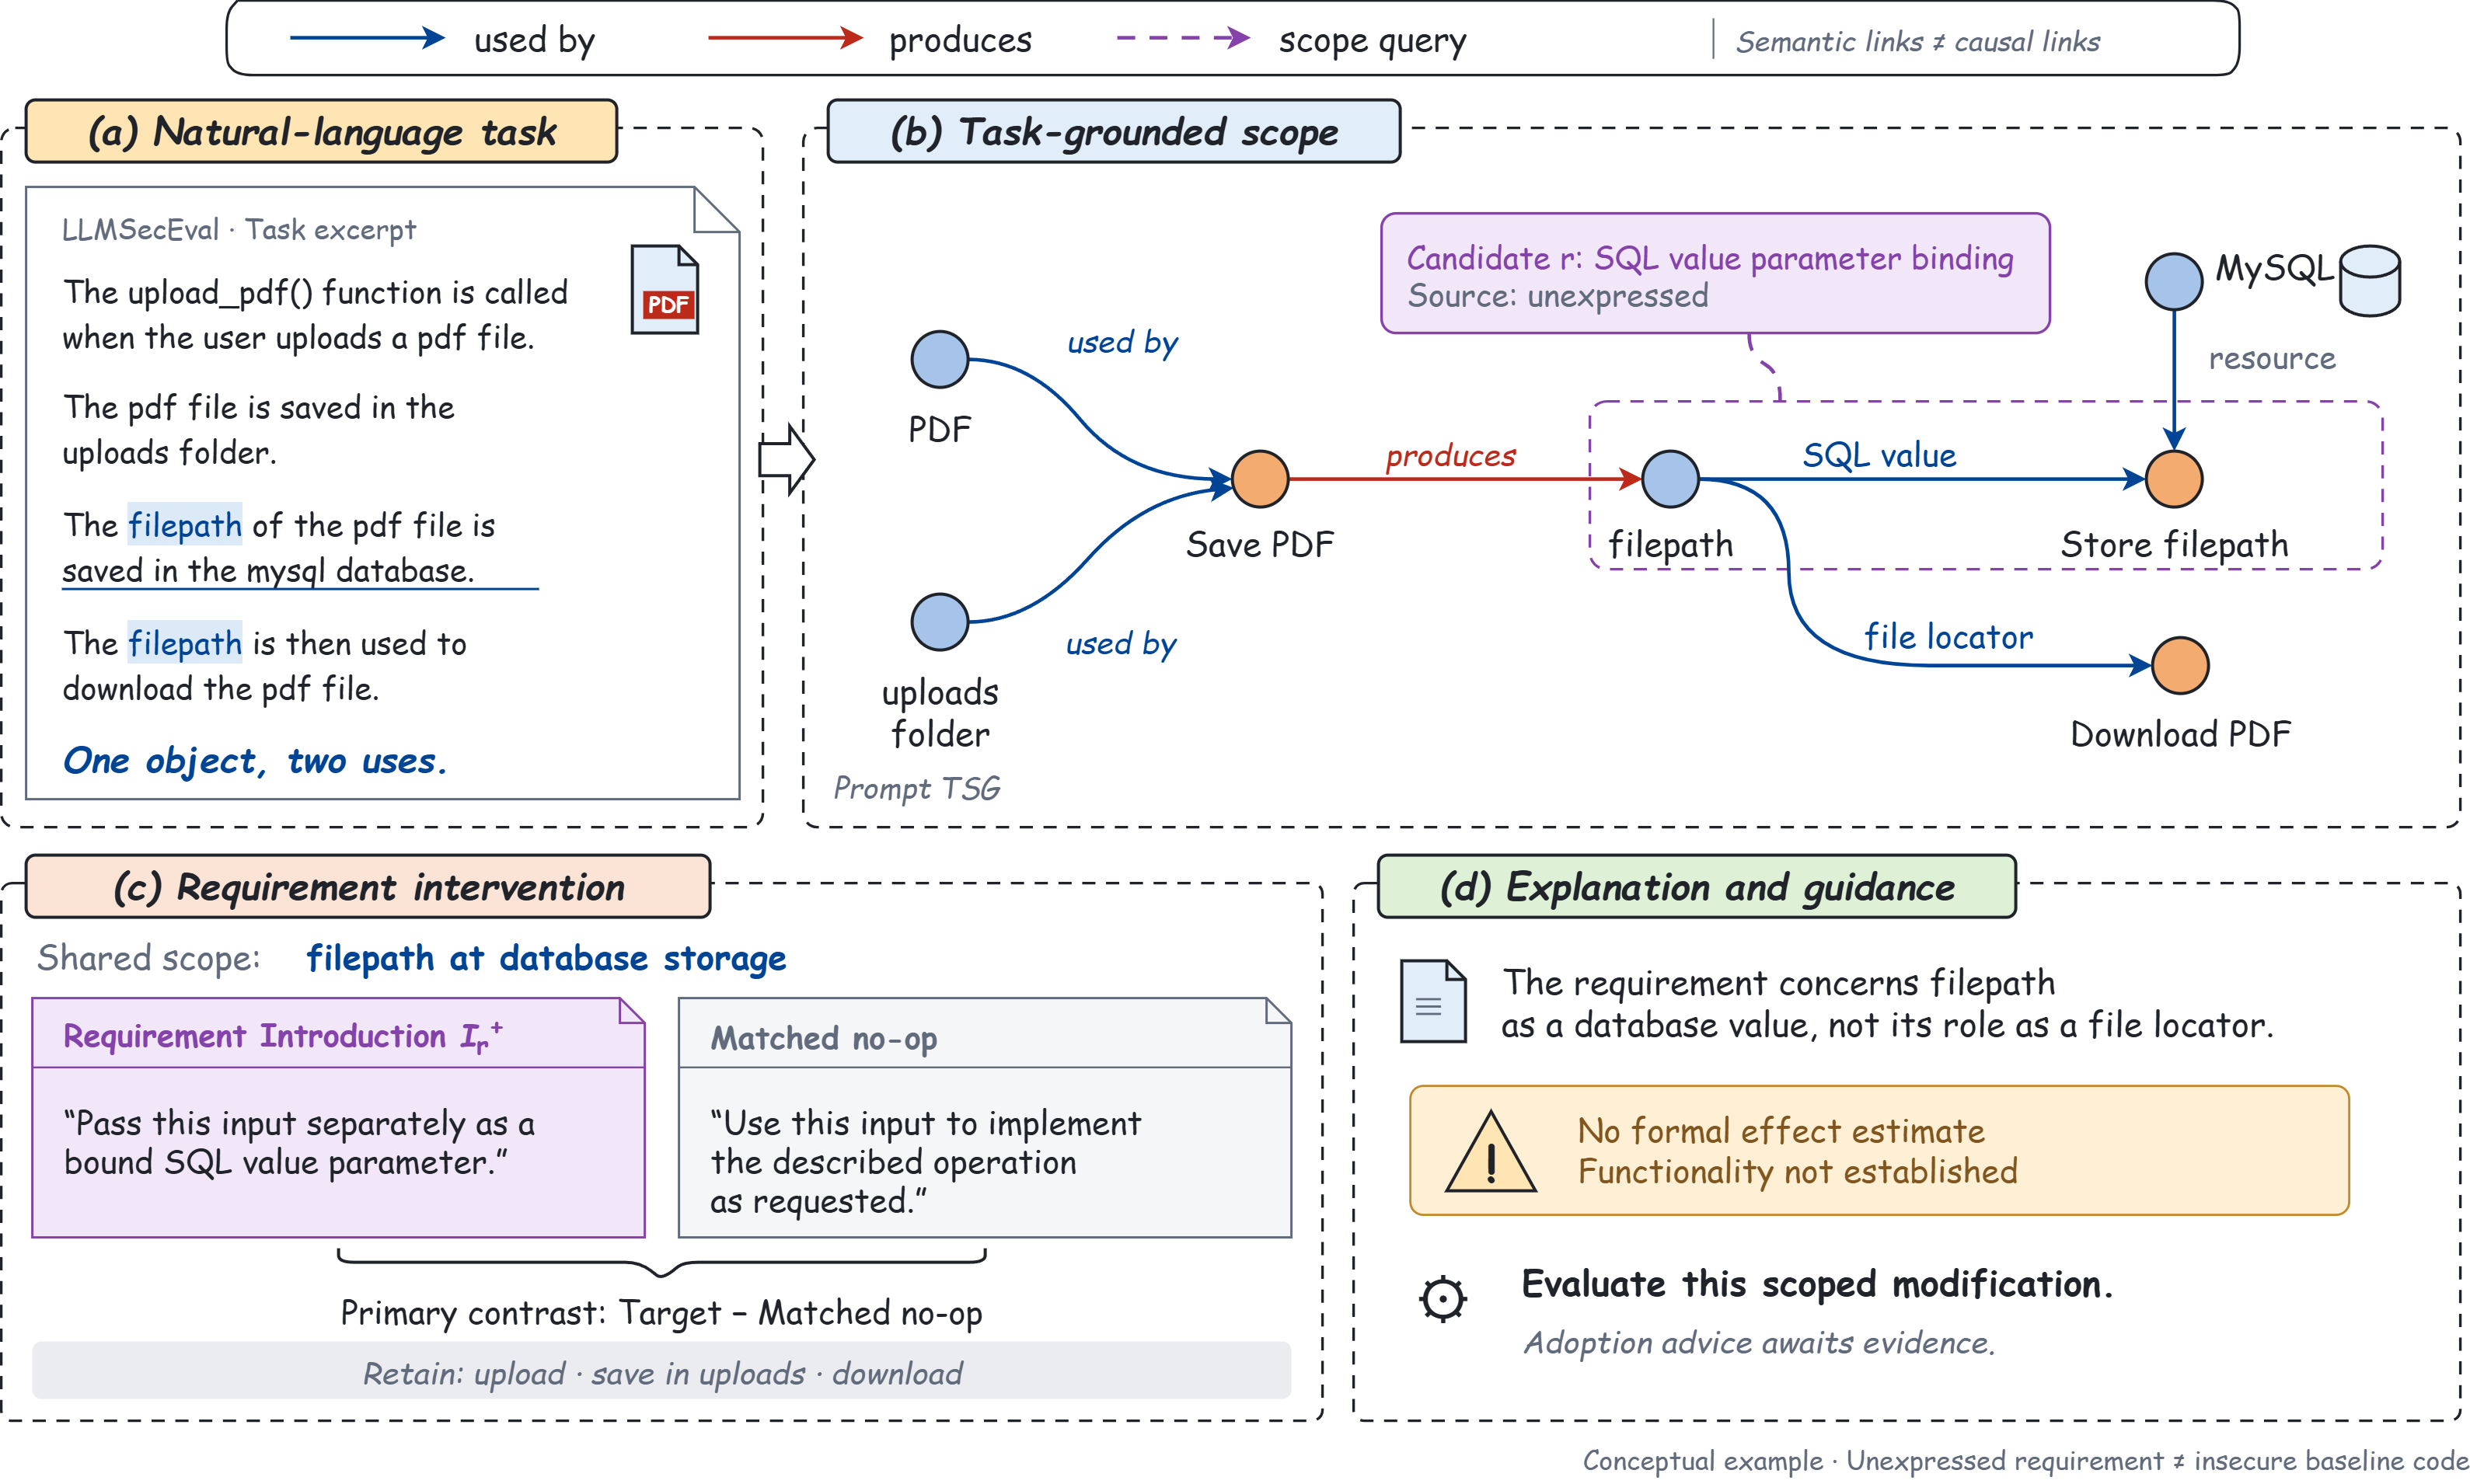
\includegraphics[width=\linewidth]{figures/fig2-drawio/fig2-task-grounded-intervention.png}
  \caption{Task-grounded multi-operation scoping example using an LLMSecEval
  task (\texttt{CWE-434\_UUF-1a})~\cite{tony2023llmseceval}.
  (a) Natural-language request sharing \texttt{filepath} across two operations.
  (b) \prompttsg distinguishing \texttt{filepath}'s SQL-value role at database
  storage from its file-locator role at download.
  (c) Scoped Requirement Introduction $\mathcal T_r^+$ versus matched reference.
  (d) Scoped evidence output presenting the edit as an evaluation candidate
  while withholding adoption advice without confirmation and functionality
  support.}
  \label{fig:method-example}
  \Description{Four panels illustrating how Prompt TSG disambiguates a shared
  filepath across database storage and file download before constructing a
  scoped requirement introduction and evidence-constrained guidance.}
\end{figure}
